% The master copy of this demo dissertation is held on my filespace
% on the cl file serve (/homes/mr/teaching/demodissert/)

% Last updated by MR on 2 August 2001

\documentclass[12pt,twoside,notitlepage]{report}

\usepackage{a4}
\usepackage{verbatim}
\usepackage{units}
\usepackage{hyperref}
\usepackage{array}
\usepackage{listings}
\usepackage{parskip}
\usepackage{color}
\usepackage[noline,plain]{algorithm2e}
\usepackage{minibox}
\usepackage{amsfonts}
\usepackage{graphicx}
\usepackage{float}

% \usepackage{dejavu}
% \usepackage{courier}
\usepackage[T1]{fontenc}

\input{epsf}                            % to allow postscript inclusions
% On thor and CUS read top of file:
%     /opt/TeX/lib/texmf/tex/dvips/epsf.sty
% On CL machines read:
%     /usr/lib/tex/macros/dvips/epsf.tex


\raggedbottom                           % try to avoid widows and orphans
\sloppy
\clubpenalty1000%
\widowpenalty1000%

\addtolength{\oddsidemargin}{6mm}       % adjust margins
\addtolength{\evensidemargin}{-8mm}

\renewcommand{\baselinestretch}{1.1}    % adjust line spacing to make
                                        % more readable
                                        
\newcommand{\strAuthor}{David Brazdil}
\newcommand{\strCollege}{Trinity Hall}
\newcommand{\strTitle}{Taint-based Data Flow Analysis on Android}
\newcommand{\strExamination}{Computer Science Tripos, Part II}
\newcommand{\strYear}{June 2013}
\newcommand{\strSupervisor}{Dr A. Beresford}

\newcommand{\centerbox}[1] {
	\begin{center}
		\minibox{#1}
	\end{center}
}
\newcommand{\asm}[1] {\small{\textsf{#1}}}
\newcommand{\asmOrig}[1] {\textbf{\asm{#1}}}
\newcommand{\asmTab} {\hspace{10pt}}

\newcommand{\tick}{$\checkmark$}
\newcommand{\cross}{$\times$}

\setlength{\intextsep}{10pt}

\title{\strTitle}
\author{\strAuthor}

\begin{document}

\bibliographystyle{plain}

\lstset{
	language=Java,
	tabsize=2,
	basicstyle=\ttfamily\scriptsize,
	escapeinside=\`\`, %{\%*}{*)},
	captionpos=b,
	keywordstyle=\color[rgb]{0,0,1},
    commentstyle=\color[rgb]{0.133,0.545,0.133},
    stringstyle=\color[rgb]{0.627,0.126,0.941},	
}

%%%%%%%%%%%%%%%%%%%%%%%%%%%%%%%%%%%%%%%%%%%%%%%%%%%%%%%%%%%%%%%%%%%%%%%%
% Title


\pagestyle{empty}

\hfill{\LARGE \bf \strAuthor}

\vspace*{60mm}
\begin{center}
\Huge
{\bf \strTitle} \\
\vspace*{5mm}
Diploma in Computer Science \\
\vspace*{5mm}
Trinity Hall \\
\vspace*{5mm}
\today  % today's date
\end{center}

\cleardoublepage

%%%%%%%%%%%%%%%%%%%%%%%%%%%%%%%%%%%%%%%%%%%%%%%%%%%%%%%%%%%%%%%%%%%%%%%%%%%%%%
% Proforma, table of contents and list of figures

\setcounter{page}{1}
\pagenumbering{roman}
\pagestyle{plain}

\chapter*{Proforma}

{\large
\begin{tabular}{ll}
Name:               & \bf \strAuthor                       \\
College:            & \bf \strCollege                     \\
Project Title:      & \bf \strTitle \\
Examination:        & \bf \strExamination, \strYear        \\
Word Count:         & \bf 1587\footnotemark[1] \\
Project Originator: & \strSupervisor                    \\
Supervisor:         & \strSupervisor                    \\ 
\end{tabular}
}
\footnotetext[1]{This word count was computed
by {\tt detex -n diss.tex | tr -cd '0-9A-Za-z $\tt\backslash$n' | wc -w}
}
\stepcounter{footnote}


\section*{Original Aims of the Project}

To write a demonstration dissertation\footnote{A normal footnote without the
complication of being in a table.} using \LaTeX\ to save
student's time when writing their own dissertations. The dissertation
should illustrate how to use the more common \LaTeX\ constructs. It
should include pictures and diagrams to show how these can be
incorporated into the dissertation.  It should contain the entire
\LaTeX\ source of the dissertation and the Makefile.  It should
explain how to construct an MSDOS disk of the dissertation in
Postscript format that can be used by the book shop for printing, and,
finally, it should have the prescribed layout and format of a diploma
dissertation.


\section*{Work Completed}

All that has been completed appears in this dissertation.

\section*{Special Difficulties}

Learning how to incorporate encapulated postscript into a \LaTeX\
document on both CUS and Thor.
 
\newpage
\section*{Declaration}

I, [Name] of [College], being a candidate for Part II of the Computer
Science Tripos [or the Diploma in Computer Science], hereby declare
that this dissertation and the work described in it are my own work,
unaided except as may be specified below, and that the dissertation
does not contain material that has already been used to any substantial
extent for a comparable purpose.

\bigskip
\leftline{Signed [signature]}

\medskip
\leftline{Date [date]}

\cleardoublepage

\tableofcontents

\listoffigures

\newpage
\section*{Acknowledgements}

This document owes much to an earlier version written by Simon Moore
\cite{moore95}.  His help, encouragement and advice was greatly 
appreciated.

%%%%%%%%%%%%%%%%%%%%%%%%%%%%%%%%%%%%%%%%%%%%%%%%%%%%%%%%%%%%%%%%%%%%%%%
% now for the chapters

\cleardoublepage        % just to make sure before the page numbering
                        % is changed

\setcounter{page}{1}
\pagenumbering{arabic}
\pagestyle{headings}

\chapter{Introduction}


\cleardoublepage
\chapter{Preparation}

\section{Dalvik Virtual Machine}

Dalvik is an open-source virtual machine and an essential component of the Android operating system. It was developed specifically for use on mobile devices such as smartphones and tablets, and its design was optimised for running on battery-powered systems with low-performance processor and limited memory. 

Built around the Apache Harmony project, Dalvik runs programs that are compatible with a subset of the Java runtime framework. Applications for Dalvik are therefore typically written in Java, compiled to a set of JVM bytecode \emph{.class} files, and then converted to a single Dalvik-compatible \emph{.dex} file using tools in the Android SDK. Thanks to Dalvik's JIT compiler, applications for Android run almost natively while staying independent of the underlying architecture.

\subsection{Application Package Files}

Applications for Android are distributed in Application Package files (APK). These are ZIP files signed by the publisher, which contain:
\begin{itemize}
\item the executable \textbf{classes.dex} file
\item application resources (images, UI layouts, ...)
\item native code binaries
\item manifest
\end{itemize}

The compulsory manifest file contains essential information about the application to the operating system. Among other things, this includes its unique package name, list of permissions requested by the application, and a list of all its entry points.

\subsection{Bytecode}

\subsubsection{Registers}

Unlike the stack-based JVM, Dalvik uses a register-based programming model with 32-bit register width and variable-length instructions. 64-bit values are stored in two adjecent registers.

Each method can use up to 65,536 virtual registers. Actual mapping to hardware registers depends on the machine architecture. On a typical Android device, the first 16 virtual registers would map to the 16 registers available in the ARM instruction set, and rest would be stored in memory. Depending on their length, instructions can address either the first 16, first 256, or all 65k virtual registers. If an instruction needs to address a register out of the available range, the register contents are expected to get moved to a lower register first.

\subsubsection{Syntax of Assembly}
Assembly syntax used in the code examples and instrumentation rules of this dissertation is mostly based on the official Dalvik assembly. It follows the \emph{dest-then-source} ordering of arguments, and instructions can contain immediate values, e.g. the instruction
		\centerbox{
			\asm{add-int/lit16 v2, v8, \#1234}
		}
adds 1234 to the value of register 8, and stores the result into register 2. 

Written rules of taint propagation will treat registers like variables. For example the following piece of code retrieves an element of an array pointed to by \verb$vArray$, and multiplies it by three.
	\begin{figure}[H]
		\centerbox{
			\asm{aget-int vElement, vArray, vIndex} \\
			\asm{mul-int/lit16 vResult, vElement, \#3}
		}
	\end{figure}

For better clarity, the first letters of register names will represent their origin. Names of registers used in the original code will start with \verb$r$, registers added for tainting with \verb$t$, and other with \verb$p$.

Register pairs forming a wide argument will be separated by a bar.
	\begin{figure}[H]
		\centerbox{
			\asm{move-wide rTo1 | rTo2, rFrom1 | rFrom2}
		}
	\end{figure}

\subsubsection{Instruction Variants}

To achieve better code density, some Dalvik instructions come in several variants. They are semantically equivalent but they differ in size. A good example of this is the \verb$const$ instruction. Its variant \verb$const/16$ stores a 16-bit constant into a register addressed by an 8-bit number, fitting into 4 bytes. On the other hand, \verb$const/4$ fits into 2 bytes, but can only address registers in the 4-bit range and carry a 4-bit constant.

All variants of semantically equivalent instructions are parsed as the same instruction type in Dexter, and thus will be referred to  by the same name. During the reassembly phase, Dexter automatically outputs the most optimised variant of the instruction possible.

\section{Data Flow Analysis}

\subsection{Taint Tags}

Different taint tracking systems choose different ways of representing taint tags. This fundamental choice has large effect on the overall design of the system, its capabilities and limits, as well as performance and memory overhead. The authors of TaintDroid decided to store taint tags as 32-bit integers where each bit represents one source of sensitive data. This is a very efficient and compact format, sufficient for the purposes of TaintDroid, but quickly reaches its limits as the functionality is extended. One of the challenges faced by the CleanOS project, which builds on TaintDroid, was the neccessity to potentially track millions of taint sources. Their solution alters TaintDroid to store taint as a 32-bit pointer into an SQL database, which increases the number of trackable sources, but significantly impedes performance at the same time. 

For the sake of simplicity, Dexter adopts the same tag representation as TaintDroid, with one slight modification. As will be demonstrated later, identification of some sinks relies on distinguishing how certain objects were created. Hence upper bits of the tags are reserved to represent the potential of an object to create a particular type of sink if passed as an argument to some API calls. The meaning of each bit being set is summarized in table ~\ref{table:TaintTagStorage_BitMeaning}.

\begin{table}
	\begin{center}
	\begin{tabular}{|c|l|l|}
		\firsthline
		\textbf{Bit} & \textbf{Constant name}        & \textbf{Description} \\
		\hline
		0            & \verb$TAINT_SOURCE_CONTACTS$  & contact information \\
		1            & \verb$TAINT_SOURCE_SMS$       & text message data \\
		2            & \verb$TAINT_SOURCE_CALL_LOG$  & call history information \\
		3            & \verb$TAINT_SOURCE_LOCATION$  & location information \\
		4            & \verb$TAINT_SOURCE_BROWSER$   & browser data, e.g. bookmarks \\
		5            & \verb$TAINT_SOURCE_DEVICE_ID$ & device ID, e.g. IMEI/phone number \\
		\hline
		29           & \verb$TAINT_SINK_FILE$        & file-system sink \\
		30           & \verb$TAINT_SINK_NET$         & network sink \\
		31           & \verb$TAINT_SINK_OUT$         & standard console output sink \\
		\lasthline
	\end{tabular}
	\end{center}
	\caption{Meanings of bit flags of taint tags}
	\label{table:TaintTagStorage_BitMeaning}
\end{table}

\subsection{Tag Storage}

To store and propagate taint tags, Dexter must build an attribute system inside the modified application, so that every piece of data accessible by the executable code can carry one if necessary. The way tags are stored differs for objects and for primitives. The crutial difference between these is that when a primitive is copied, operations on one of the copies do not effect the other ones. When a reference to an object is copied, operations on one of the copies is visible by dereferencing any of them.

\subsubsection{Objects}

Objects are uniquely defined by the pointer to their place in memory. Dexter therefore allows to store one taint tag per object reference by adding a globally accessible hash map. The only two supported operation are:
\begin{description} 
\item \verb$int get(Object obj)$ \\
Returns the taint tag of given object. Returns zero when \verb$obj == null$.
\item \verb$void set(int taint, Object obj)$ \\
Adds taint to \verb$obj$ by OR-ing its existing entry with the first parameter. Does nothing when \verb$obj == null$.
\end{description}

In the following sections, the \verb$taint-get$ and \verb$taint-set$ pseudo-instructions (explained in section ~\ref{section:Code_Pseudoinstructions}) will be used as a shorthand for calling the \verb$get$ and \verb$set$ methods of the hash map. Their syntax follows the signatures above:

	\begin{figure}[H]
		\centerbox{
			\asm{taint-get vResult, vObject} \\
			\asm{taint-set vAddedTaint, vObject}
		}
	\end{figure}

\subsubsection{Primitives}

\label{section:TaintStorage_Primitives}

In the case of primitives, Dexter needs to create taint storage space everywhere where a primitive might be stored, i.e. method code registers, and class fields and arrays of primitive types. Primitives can also be stored as method arguments, but this will be covered in section ~\ref{section:TaintPropagation_MethodCalls}.

\begin{itemize}

\item \textbf{method code registers} \\
For every register that appears in the original method code, Dexter creates a new one that can be used for storing taint. This effectively doubles the number of used registers, which is why Dexter needs to perform constraint-solving register colouring during the assembly phase. Otherwise some instructions might not be able to address these new registers.

\item \textbf{internal class fields} \\
Classes defined inside the application's DEX file can be fully modified by Dexter. Hence, for every field of primitive type, new field of type \verb$int$ is created, with a name that will not clash with any of the existing fields.

\item \textbf{external class fields} \\
Extra fields cannot be inserted into class defined outside the scope of the instrumented application, and therefore a different approach must be adopted. 
\begin{itemize}
\item static fields \\
A special class is created inside the application which contains one field of type \verb$int$ per every external static field that is accessed by the application. Taint tags are stored in these associated fields.

\item instance fields \\
It would be possible to create taint storage for every field inside every instance of an external class, for example by creating one global map from object references to integers per every accessed external instance field. However, it will be shown that it is actually necessary to assign the taint to the object itself, and thus storage space for these fields is not needed.

\item \textbf{arrays} \\
In Dexter's taint propagation logic, primitive arrays are equivalent to external instance fields, and therefore only one taint tag per array is stored.

\end{itemize}

\end{itemize}


\subsection{Basic Taint Propagation Rules}

Once taint storage is created, Dexter can insert extra instructions that will propagate taint as data are used. Dalvik supports 217 different opcodes, but these can be divided into groups that share the same propagation logic. General rule of thumb is that for every instruction, taint of all arguments should be acquired from their respective storage spaces, combined and stored to the taint storage of the result. Therefore, only a handful of examples will be presented here to illustrate the principle and to explain some of the subtleties.

The following snippets of Dalvik assembly will always show the original instruction in bold typeface and the inserted instructions in regular font. 

\subsubsection{Constants}

Constants are created without any taint flags set. Zero should therefore be stored in the appropriate taint register.

	\begin{figure}[H]
		\centerbox{
			\asmOrig{const rTo, \#num} \\
			\asm{const tTo, \#0}
		}
	\end{figure}

\subsubsection{Instructions Combining Taint}

Arithmetic instructions are the simplest example of taint tag combination. Tags of the operands are OR-ed and this combined tag is assigned to the result of the original instruction.

	\begin{figure}[H]
		\centerbox{
			\asmOrig{add-int rResult, rOpA, rOpB} \\
			\asm{or-int tResult, tOpA, tOpB}
		}
	\end{figure}

\subsubsection{Instructions Operating on Wide Registers}

Taint for 64-bit primitives stored in wide register pairs is only stored in the taint register associated with the higher of the two original registers. This is safe because accessing only one of the registers as a single-width register is an illegal operation. Class containing such instruction will be rejected by Dalvik's preload class verifier.

	\begin{figure}[H]
		\centerbox{
			\asmOrig{add-long rResult1 | rResult2, rOpA1 | rOpA2, rOpB1 | rOpB2} \\
			\asm{or-int tResult1, tOpA1, tOpB1}
		}
	\end{figure}

\subsubsection{Instructions Throwing Exceptions}

Some of Dalvik instructions can throw exceptions, depending on the values of arguments passed to them. This is a form of implicit data flow and could potentially leak some sensitive data. For example, integer division will throw \verb$ArithmeticException$ if and only if the divisor is equal to zero, making this information deducible from the fact that the exception was thrown. Dexter deals with this by wrapping every such instruction in a try block, catching the exception, passing the correct taint to it and then throwing it again.

	\begin{figure}[H]
		\centerbox{
			\asm{TRY (ArithmeticException $\Rightarrow$ CATCH\_ABC) \{} \\
			\asmTab\asmOrig{div-int rResult, rOpA, rOpB} \\
			\asmTab\asm{or-int tResult, tOpA, tOpB} \\
			\asmTab\asm{goto LABEL\_XYZ} \\
			\asm{\}} \\
			\asm{CATCH\_ABC:} \\
			\asm{move-exception pException} \\
			\asm{taint-set tOpB, pException} \\
			\asm{throw pException} \\	
			\asm{LABEL\_XYZ:}
		}
	\end{figure}

% \subsubsection{Instructions Operating on External Instance Fields}

% Data stored in instance fields defined in external classes can be accessed by untrackable code. 

% In previous examples, inserted instructions only addressed taint registers. When arguments are reference-based, methods of the hash map are called and these arguments are passed to them. However, they might not be available after the original instruction any more, because they can be overwritten by the instruction's result. 


% This problem is illustrated by the following rule, in which 

% This problem is illustrated by the following rule, in which the original instruction retrieves a reference stored in an external instance class field of some object. Since fields defined externally could 

% Since the object might have been assigned taint after the reference was already stored in its field, taint of the object must be propagated to the result. In case \verb$rValue$ and \verb$rObject$ map to the same register, taint of the object must be retrieved before the original instruction. And because the value of the field is not known before, calls to \verb$taint-set$ must be added after the instruction.

% \centerbox{
% 	\asm{taint-get tObject, rObject} \\
% 	\asmOrig{iget-obj rValue, rObject, \#fieldID} \\
% 	\asm{taint-set tObject, rValue}
% }

% In the opposite direction, the rule differs for fields defined internally and externally. Because externally defined fields could be accessed by untrackable code, taint must be assigned to the object itself, rather than just the field as in the internal case, so that when the object is passed to external code, it is known that it contains sensitive data. Hence the needlessness for storage space for external instance fields mentioned in section ~\ref{section:TaintStorage_Primitives}.

% \centerbox{
% 	\asm{taint-get tValue, rValue} \\
% 	\asmOrig{iput-obj rValue, rObject, \#externalFieldID} \\
% 	\asm{taint-set tValue, rObject}
% }

% \subsubsection{Instructions Operating on Arrays}

% Arrays are treated in a similar way to external class fields. When retrieving an element, it has to inherit the taint of the array, as well as the taint of the value used as index. Putting a value into an array requires passing its taint and the taint of the index to the array object.


\subsection{Inter-Procedural Taint Propagation}
\label{section:TaintPropagation_MethodCalls}

While the previous examples of propagation rules only dealt with taint propagation within the scope of one instrumented method, this section will focus on the propagation of taint when method calls are involved. 

The five types of method invocation supported by Dalvik are listed in table ~\ref{table:TaintPropagation_MethodCallTypes}. Instrumentation of each of these will vary in slight details, but for propagation logic it will be more important to know whether a method call jumps to another place inside the executable file or whether it jumps out of it, into untrackable code. These two cases will be handled in an entirely different manner. 

\begin{table}
	\begin{center}
	\begin{tabular}{|l|c|l|}
		\firsthline
		\textbf{Opcode}         & \footnotesize{\textbf{vtable}} & \textbf{Usage} \\
		\hline
		\verb$invoke-direct$    & \cross          & method declared \verb$private$ or a constructor \\
		\verb$invoke-static$    & \cross          & method declared \verb$static$ \\
		\hline
		\verb$invoke-virtual$   & \tick           & standard virtual method call \\
		\verb$invoke-interface$ & \tick           & method declared in an interface \\
		\verb$invoke-super$     & \tick           & call to closest parent implementing the method \\
		\lasthline
	\end{tabular}
	\end{center}
	\caption{Method call types supported by Dalvik}
	\label{table:TaintPropagation_MethodCallTypes}
\end{table}

\subsubsection{Destination Decidability}

Deciding the destination of a method call is simplest in the case of a \verb$-direct$ invoke instruction. The method signature, passed as an argument to the instruction, always contains the name of the class the method is implemented in. Therefore, \verb$invoke$ instruction will perform an internal jump if and only if the referenced class is defined internally.

Only slightly more complicated is the case of a \verb$-static$ call. The reason being that the method might not be implemented directly in the referenced class, but rather inherited from the parent. Checking that the referenced class is internal is thus insufficient. Dexter must check that this class indeed implements a method of given signature and if not, recursively explore the parent of the class. 

All the other calls rely on dynamic dispatch. Since they are very similar, only the standard \verb$-virtual$ case will be discussed here. We will illustrate the decision logic on an example of a class hierarchy depicted in figure ~\ref{fig:TaintPropagation_DestDecision_ClassHierarchy}. Assume the instruction expects an object of type G. From the nature of virtual calls, we know that the invoked method is declared either in the referenced class itself or in one of its parents, and implemented in any of the children of the declaring class. Assume it is declared in B and implemented in B, E, F and H. Table ~\ref{table:TaintPropagation_DestDecision_ClassHierarchy_Destinations} summarizes which implementation will be called for all possible types of the first argument (\verb$this$) passed to the instruction. It is obvious that not all the implementations of the method can be called by this instruction. In general, these are implementations in the referenced class, in any of the children, and in the closest parent, i.e. B and E in this case. If these classes are all internal or all external, the destination of the call is decidable statically. 

\begin{figure}
	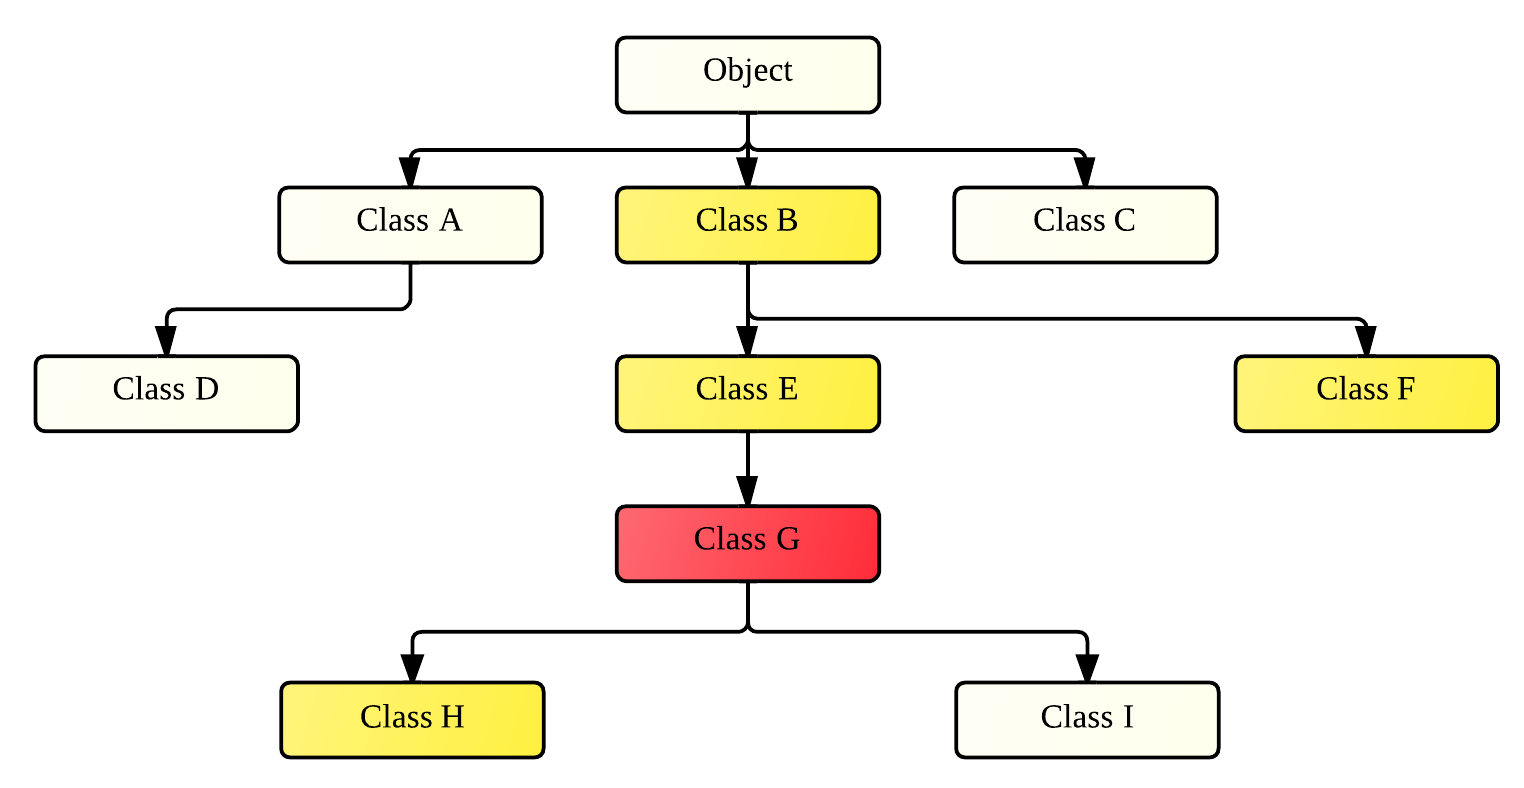
\includegraphics[width=\textwidth]{figs/fig_virtual_call_tree.png}
	\caption{Example class hierarchy}
	\label{fig:TaintPropagation_DestDecision_ClassHierarchy}
\end{figure}

\begin{table}
	\begin{center}
	\begin{tabular}{|c|c|}
		\firsthline
		\textbf{Type of} \verb$this$ & \textbf{Called implementation} \\
		\hline
		G & E \\
		H & H \\
		I & E \\
		\lasthline
	\end{tabular}
	\end{center}
	\caption{Call destinations for different types of \texttt{this} argument.}
	\label{table:TaintPropagation_DestDecision_ClassHierarchy_Destinations}
\end{table}

If the algorithm above cannot decide the destination of a call, code could be further analysed to narrow down the number of callable implementations, e.g. by performing reachability analysis on the type of the instruction's first argument. However, it will always be possible to produce code with a statically undecidable call. Then it is necessary to instrument the code in a way that the decision can be made at runtime using reflection. Dexter adds a special annotation to every method defined inside the application. Consequently, internal and external implementations can be distinguished at runtime by reflectively finding the target method and checking whether it carries the annotation or not. Slight subtlety comes from the fact that the reflexive API handles public and non-public instance methods differently. Code for non-public methods is shown in listing ~\ref{listing:TaintPropagation_MethodCall_DestDecidability_NonPublic}. Instrumentation for public methods uses \verb$Class.getMethod$ to get \verb$m$ and does not need to iterate through parents until an implementation is found. It is, nonetheless, obvious that these are both very expensive operations. 

\begin{figure}
	\lstset{
		caption = {Destination-deciding instrumentation for non-public methods},
		label = {listing:TaintPropagation_MethodCall_DestDecidability_NonPublic}
	}
	\begin{lstlisting}
	// original code: obj.methodName(arg1, arg2, ..., argN)
	Class c = obj.getClass();
	Class[] argTypes = new Class[] { arg1.class, ..., argN.class };

	Method m = null;
	while (m == null) {
		try {
	 		m = c.getDeclaredMethod("methodName", argTypes);
	 	} catch (NoSuchMethodException e) {
	 		c = c.getSuperclass();
	 	}
	}

	Annotation a = m.getAnnotation(InternalMethodAnnotation.class);
	if (a == null) {
		// external call
		obj.methodName(arg1, ..., argN);
	} else {
		// internal call
		obj.methodName(arg1, ..., argN);
	}
	\end{lstlisting}
\end{figure}

\subsection{Internal Method Calls}



\subsection{External Method Calls}

\subsection{Propagation Logic for External Fields}

\subsection{Holes in Propagation Logic}

\section{Source/Sink Identification}

\subsection{Sources}

\subsection{Sinks}

\section{Requirements Analysis}
look at AdCache

\section{Software Engineering}

\subsection{Approach}

\subsection{Android Genome Project}

\section{Tools}

\subsection{Programming Languages}

\subsection{Software Libraries}

\subsection{Android SDK}

\subsection{Version Control}

\subsection{Evaluation Tools}

\cleardoublepage
\chapter{Implementation}

\label{section:Code_Pseudoinstructions}


\cleardoublepage
\chapter{Evaluation}


\cleardoublepage
\chapter{Conclusion}



\cleardoublepage

%%%%%%%%%%%%%%%%%%%%%%%%%%%%%%%%%%%%%%%%%%%%%%%%%%%%%%%%%%%%%%%%%%%%%
% the bibliography

\addcontentsline{toc}{chapter}{Bibliography}
\bibliography{refs}
\cleardoublepage

%%%%%%%%%%%%%%%%%%%%%%%%%%%%%%%%%%%%%%%%%%%%%%%%%%%%%%%%%%%%%%%%%%%%%
% the appendices
\appendix

\chapter{Latex source}

\section{diss.tex}
{\scriptsize\verbatiminput{diss.tex}}

\section{proposal.tex}
{\scriptsize\verbatiminput{proposal.tex}}

\section{propbody.tex}
{\scriptsize\verbatiminput{propbody.tex}}



\cleardoublepage

\chapter{Makefile}

\section{\label{makefile}Makefile}
{\scriptsize\verbatiminput{makefile.txt}}

\section{refs.bib}
{\scriptsize\verbatiminput{refs.bib}}


\cleardoublepage

\chapter{Bytecode for the Dalvik VM}

% \input{dalvik-bytecode}


\cleardoublepage

\chapter{Project Proposal}


% Draft #1 (final?)

\vfil

\centerline{\Large Computer Science Project Proposal}
\vspace{0.4in}
\centerline{\Large How to write a dissertation in \LaTeX\ }
\vspace{0.4in}
\centerline{\large M. Richards, St John's College}
\vspace{0.3in}
\centerline{\large Originator: Dr M. Richards}
\vspace{0.3in}
\centerline{\large 14$^{th}$ October 2011}

\vfil


\noindent
{\bf Project Supervisor:} Dr M. Richards
\vspace{0.2in}

\noindent
{\bf Director of Studies:} Dr M. Richards
\vspace{0.2in}
\noindent
 
\noindent
{\bf Project Overseers:} Dr~F.~H.~King  \& Dr~A.~W.~Moore


% Main document

\section*{Introduction, The Problem To Be Addressed}


Many students write their CST dissertations in \LaTeX\ and
spend a fair amount of time learning just how to do that. The purpose of 
this project is to write a demonstration dissertation that explains in
detail how it done.  

This core proposal document will be augmented by a separately-printed
cover sheet at the front and a resource form at the end.  Additional
sheets for risk assessment and human resources may also need to be included.

This document will repeat much of the material that is summarised on the additional sheets.

\section*{Starting Point}

{\em Describe existing state of the art, previous work in this area, libraries and databases to be used.
Describe the state of any existing codebase that is to be built on.  }

I am already able to write prose using the English language. I have an online dictionary. etc..

\section*{Resources Required}

{\em A note of the resources required and confirmation of access.}

For this project I shall mainly use my own quad-core computer that runs Fedora Linux. Backup
will be to github and/or to an SVN repository on an external hard disk that is dumped to writable CD/DVD media.
I have another similar computer to hand should my main machine suddenly fail.
I require no other special resources.

\section*{Work to be done}

{\em Describe the technical work.}

The project breaks down into the following sub-projects:

\begin{enumerate}

\item The construction of a skeleton dissertation with the required 
structure. This involves writing the Makefile and makeing dummy files
for the title page, the proforma, chapters 1 to 5, the appendices and
the proposal.

\item Filling in the details required in the cover page and proforma.

\item Writing the contents of chapters 1 to 5, including examples
of common \LaTeX\ constructs.

\item Adding a example of how to use floating figures and encapsulated
postscript diagrams.

\end{enumerate}

\section*{Success Criterion for the Main Result}


The project will be a success if I have a completed dissertation with the correct chapter
titles and I have achieved my other success criterion, which is to blah ...



\section*{Possible Extensions}

{\em Potential further envisaged evaluation metrics or extensions.}

If I achieve my main result early I shall try the following alternative experiment or method of evaluation ...


\section*{Timetable: Workplan and Milestones to be achieved.}


{\em Perhaps list ten or so  two-week work-packages.}

Planned starting date is 16/10/2011.

\begin{enumerate}

\item {\bf Michaelmas weeks 2-4} Learn to use X. Read book Y. Read papers Z.

\item {\bf Michaelmas weeks 5-6} Do preliminary test of Q.

\item {\bf Michaelmas weeks 7-8} Start implementation of main task A.

\item {\bf Michaelmas vacation} Finish A and start main task B.

\item {\bf Lent weeks 0-2} Write progress report. Generate corpus of test examples. Finish task B.  

\item {\bf Lent weeks 3-5} Run main experiments and achieve working project.

\item {\bf Lent weeks 6-8} Second main deliverable here.

\item {\bf Easter vacation:} Extensions and writing dissertation main chapters.

\item {\bf Easter term 0-2:}  Further evaluation and complete dissertation.

\item {\bf Easter term 3:} Proof reading and then an early submission so as to concentrate on examination revision.

\end{enumerate}


 



\end{document}
